% DO NOT COMPILE THIS FILE DIRECTLY!
% This is included by the other .tex files.

\begin{frame}[t,plain]
\titlepage
\end{frame}

\begin{frame}
    \frametitle{Log4J exploitation lab}
    The goal of this lab is to analyze a network capture evidence file, encode, and share the information following successful exploitation by an attacker.
	\linebreak
	\linebreak
	\linebreak
    Resources:
    \begin{itemize}
        \item \href{https://github.com/MISP/misp-training-lea/tree/main/e.304-lab3-encoding-information-and-sharing-it-2/dataset/capture.pcap}{\underline{capture.pcap}}
    \end{itemize}
    Tools:
    \begin{itemize}
        \item \href{https://www.wireshark.org/}{\underline{Wireshark}}: Network protocol analyzer
        \item \href{https://github.com/skylot/jadx}{\underline{Jadx}}: Dex to Java decompiler
        \item \href{https://github.com/MISP/misp-wireshark}{\underline{misp-wireshark}}: Lua plugin to extract data from Wireshark and convert it into MISP format 
    \end{itemize}

    \note[item]{A note for the slide handout}
\end{frame}

\begin{frame}
    \frametitle{Actors}
    \href{https://github.com/MISP/misp-training-lea/tree/main/e.304-lab3-encoding-information-and-sharing-it-2/dataset/capture.pcap}{\underline{capture.pcap}} is a network capture on the eth0 interface on our Minecraft Server.
    \linebreak
    \linebreak
    {\color{blue}{\bf Minecraft Server}}
    \begin{itemize}
    	\item External IP: 44.202.61.172
	    \item Internal IP: 172.31.84.208
	    \item Version: Java Edition v1.18 
	    \item Vulnerable to \href{https://nvd.nist.gov/vuln/detail/CVE-2021-44228}{CVE-2021-44228}
    \end{itemize}
    
    External actors:
    \begin{itemize}
        \item {\color{green}{\bf Player}}
        \item {\color{red}{\bf Attacker}}
    \end{itemize}

    \note[item]{}
\end{frame}

\begin{frame}
    \frametitle{Exercise 1: Identifying the external actors }
    Using Wireshark:
    \begin{itemize}
    	\item Identify {\color{green}{\bf Player}} IP address
    	\item Identify {\color{red}{\bf Attacker}} IP address
    \end{itemize}
    \begin{center}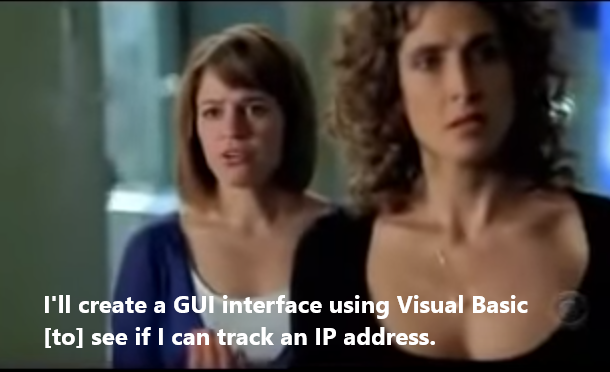
\includegraphics[scale=0.45]{../pictures/csi-meme.png}\end{center}
    \begin{center}Exercise duration: 10 minutes\end{center}
    \note[item]{Player IP: 178.249.193.69, Attacker IP: 18.212.74.161}
\end{frame}

\begin{frame}
    \frametitle{Wireshark tips}
    Statistics -> IPv4 Statistics -> All Addresses:
	\begin{center}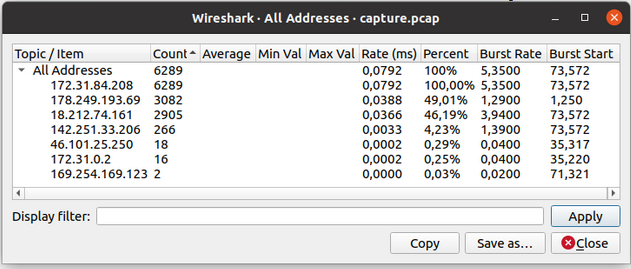
\includegraphics[scale=0.45]{../pictures/wireshark-statistics.png}\end{center}
	Useful filters:
    \begin{itemize}
    	\item ip.addr == 10.10.10.10 \&\& ip.addr == 20.20.20.20
    	\item dns.flags.rcode != 0
    \end{itemize}
    \note[item]{First one is for filtering the communication between two IP addresses only, second one shows failed dns requests, which can potentially be a C2 beaconing }
\end{frame}

\begin{frame}
    \frametitle{}


    \note[item]{A note for the slide handout}
\end{frame}
